% Provenance (never printed): the poverty strand of ../economics_series.md; World Bank
% poverty lines (PIP, June 2025 update). Brief: sources/book1/BRIEFS.md, g6-03.
% Chart data: figdata/grade-6/03-poverty (WDI SI.POV.DDAY, SI.POV.LMIC, SI.POV.UMIC, SP.POP.TOTL;
% Brenland basket and household survey from code/shared/country).
\chapter{Poverty and How It Is Counted}\label{ch:g6:poverty}

\omterm{def:g6:living-standards:income-per-person}{Income per person} tells us how much a country has on average. It does not tell
us how many of its people lack food, a roof or clothes. To know that, we must
count the poor --- and before counting them, decide who is poor. This chapter
shows how the world's poor are counted, how their number has changed since
1981, and where most of them live today.

\begin{omfigure}
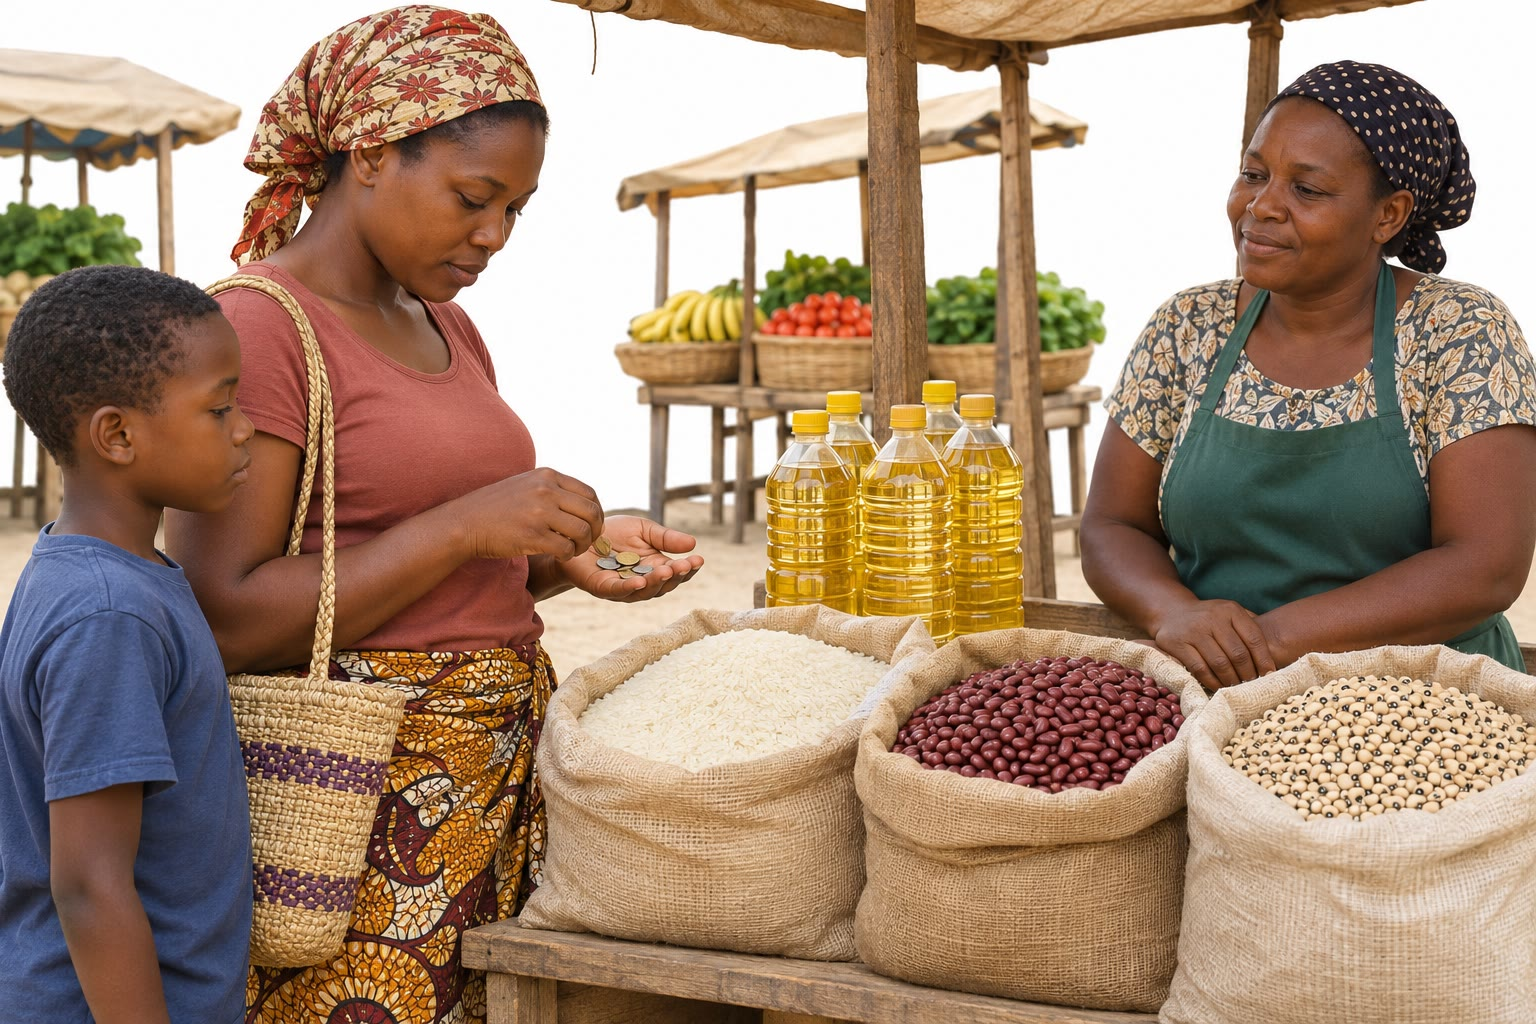
\includegraphics[width=0.62\linewidth]{images/book1/ai/g6-poverty-market.jpg}

{\small Buying rice, beans and oil at a market. A \omterm{def:g6:poverty:poverty-line}{poverty line} starts from the
price of the things a family cannot do without.}
\end{omfigure}

\begin{recall}
A \omterm{def:g6:reading-economic-charts:per-person}{per-person value} is a total divided by the number of people, and a share is
a part divided by the total, as a percentage
(\cref{def:g6:reading-economic-charts:per-person,def:g6:reading-economic-charts:share}).
\omterm{def:g6:living-standards:income-per-person}{Income per person} is measured in dollars of fixed purchasing power
(\cref{def:g6:living-standards:income-per-person}).
\end{recall}

\section{What a poverty line is}

Being poor means not having enough to meet one's basic needs: enough food to
stay healthy, a shelter, clothes, fuel to cook and clean water. To turn this
idea into a number, we price those needs.

\begin{definition}[Poverty line]\label{def:g6:poverty:poverty-line}
A \emph{poverty line}\index{poverty line} is an amount of income or spending
per person, for a day or a year. A person whose income or spending is below
the line is counted as poor. A poverty line is usually set at the cost of a
basket of basic needs: the quantities of food, shelter, clothing and other
necessities that one person needs, multiplied by their prices.
\end{definition}

\begin{omfigure}
\begin{tikzpicture}[econ, x=1cm, y=1cm]
  % invented prices for one person and one day, in dalens (sum 4.00)
  \foreach \y/\h/\c/\l in {0/2.0/omMeth/{food: 2.00}, 2.0/1.2/omDef/{shelter: 1.20},
      3.2/0.3/omProp/{clothing: 0.30}, 3.5/0.5/omThm/{fuel and water: 0.50}} {
    \fill[\c!30] (0,\y) rectangle (2.2,{\y+\h});
    \draw[\c] (0,\y) rectangle (2.2,{\y+\h});
    \node[right, font=\footnotesize] at (2.4,{\y+\h/2}) {\l};
  }
  \draw[omThm, very thick] (-0.6,4.0) -- (7.4,4.0);
  \node[above left, font=\footnotesize\bfseries, text=omThm] at (7.4,4.0) {poverty line: 4.00 dalens a day};
  \node[font=\footnotesize, align=center] at (1.1,-0.5) {a basket of needs,\\one person, one day};
  \fill[black!45] (5.6,0) rectangle (6.4,3.1);
  \node[font=\footnotesize, align=center] at (6.0,-0.5) {a person living\\on 3.10 dalens};
  \node[font=\footnotesize, text=omThm] at (6.0,3.45) {poor};
\end{tikzpicture}

{\small Pricing a basket of needs into a \omterm{def:g6:poverty:poverty-line}{poverty line} (invented prices). A person
whose income per day is below the line is counted as poor.}
\end{omfigure}

Every country that measures poverty chooses its own basket and its own prices.

\begin{definition}[National poverty line]\label{def:g6:poverty:national-poverty-line}
A country's \emph{national poverty line}\index{national poverty line} is the
\omterm{def:g6:poverty:poverty-line}{poverty line} chosen by its own statistical office, for its own people, in its
own money.
\end{definition}

National lines are very different from country to country. A rich country's
line counts as poor a family that cannot afford a heated flat, a phone and
a bus pass; a poor country's line counts as poor a family that cannot afford
enough grain. Both are reasonable for the country that draws them, but they
cannot be added up into a world count.

\section{The extreme-poverty line and the higher lines}

To count the poor of the whole world, one line must be used for everyone.

\begin{definition}[Extreme poverty]\label{def:g6:poverty:extreme-poverty}
A person lives in \emph{extreme poverty}\index{extreme poverty} when their
income or spending is below the international \omterm{def:g6:poverty:poverty-line}{poverty line}: \$3.00 a day per
person, in dollars of fixed purchasing power of 2021.
\end{definition}

\begin{measure}[The extreme-poverty line]
% ledger: g6:pip-line-3-00, g6:pip-line-2-15, g6:pip-line-23-countries, g6:pip-line-4-20, g6:pip-line-8-30
The World Bank sets the line from the \omterm{def:g6:poverty:national-poverty-line}{national poverty lines} of the poorest
countries. It takes the lines of 23 low-income countries, converts them into
dollars of the same purchasing power, and takes the middle one. So the
extreme-poverty line asks: would this person be counted as poor in one of the
poorest countries of the world? When prices are measured again, the line is
updated: it was \$2.15 a day in dollars of 2017 until 2025, and is \$3.00 in
dollars of 2021 since then. Two higher lines are also published: \$4.20 and
\$8.30 a day, built from the national lines of middle-income countries.
\end{measure}

\begin{dated}{2026}
% ledger: g6:pip-line-3-00
The international \omterm{def:g6:poverty:poverty-line}{poverty line} is \$3.00 per person per day, in dollars of
fixed purchasing power of 2021, since June 2025. Every series of this chapter
uses it, including the years before 2025: the past is counted again with the
new line, so that the years can be compared.
\end{dated}

\begin{definition}[Poverty rate]\label{def:g6:poverty:poverty-rate}
The \emph{poverty rate}\index{poverty rate} of a group is the share of its
people who are below a given \omterm{def:g6:poverty:poverty-line}{poverty line}:
\[
  \text{poverty rate} = \frac{\text{number of poor people}}{\text{number of people}}
  \times 100\,\%.
\]
A poverty rate always goes with its line: ``the rate at \$3.00 a day''.
\end{definition}

\begin{omchart}{The extreme-poverty rate of the world, 1981--2024: the share of
the world's people living on less than \$3.00 a day (dollars of 2021). The source
gives no world estimate for 2019; the line joins 2018 and 2020.}{The World Bank,
World Development Indicators, SI.POV.DDAY (Poverty and Inequality Platform)}
\begin{tikzpicture}
\begin{axis}[omtime, xmin=1980, xmax=2025, ymin=0, ymax=50,
  xtick={1980,1990,2000,2010,2020}, xlabel={Year}, ylabel={Percent of world population}]
\addplot+[mark=*, mark size=0.9pt] table[x=year, y=share]
  {figdata/grade-6/03-poverty/out/poverty_share_world.csv};
\end{axis}
\end{tikzpicture}
\end{omchart}

% figdata: poverty_share_world (1981 47.1; 1990 43.4; 2018 11.1; 2020 11.4; 2024 10.1)
In 1981, $47.1\,\%$ of the world's people lived on less than \$3.00 a day: almost
one person in two. In 2024, $10.1\,\%$ did: one person in ten. The fall was
slow in the 1980s and fast after 2000. It stopped in 2020, the year of the
pandemic, when the rate rose for the first time since 1998.

% figdata: lines_2024 (3.00 10.1; 4.20 18.2; 8.30 46.2)
With the higher lines, many more people are counted. In 2024, $18.2\,\%$ of the
world's people lived on less than \$4.20 a day, and $46.2\,\%$ on less than
\$8.30 a day. \omterm{def:g6:poverty:extreme-poverty}{Extreme poverty} has become rare in much of the world; living on a
few dollars a day has not.

\section{The share and the number}

A \omterm{def:g6:poverty:poverty-rate}{poverty rate} is a share. The number of poor people is the share multiplied by
the population, and the world's population grew from 4.5 to 8.1 billion
between 1981 and 2024. So the share and the number need not move together.

\begin{omchart}{The world's people below and above the extreme-poverty line
(\$3.00 a day, dollars of 2021), 1981--2024, in billions. The two layers add
up to the world population.}{The World Bank, World Development Indicators,
SI.POV.DDAY and SP.POP.TOTL; \omterm{def:g6:poverty:poverty-rate}{poverty rate} times population}
\begin{tikzpicture}
\begin{axis}[omtime, xmin=1981, xmax=2024, ymin=0, ymax=9, stack plots=y,
  area style, xtick={1985,1995,2005,2015}, xlabel={Year},
  ylabel={Billions of people}, legend pos=north west, legend reversed]
\addplot+[draw=omThm, fill=omThm!45] table[x=year, y=poor]
  {figdata/grade-6/03-poverty/out/poverty_count_world.csv} \closedcycle;
\addplot+[draw=omDef, fill=omDef!20] table[x=year, y=not_poor]
  {figdata/grade-6/03-poverty/out/poverty_count_world.csv} \closedcycle;
\legend{Below \$3.00 a day, Above \$3.00 a day}
\end{axis}
\end{tikzpicture}
\end{omchart}

% figdata: poverty_count_world (poor 1981 2.127, 1993 2.343, 2024 0.822; not_poor 1981 2.389, 2024 7.319;
% poor rose again 1997, 1998 and 2020 (2018 0.854, 2020 0.895); not_poor dips once, 1988-1989)
In 1981, $2.13$ billion people lived in \omterm{def:g6:poverty:extreme-poverty}{extreme poverty}. Their number rose,
with small ups and downs, until 1993, to $2.34$ billion, although the share was
mostly falling: the population grew faster than the share fell. After 1993, both
fell, with a few pauses: the number rose again in 1997 and 1998, and in 2020. In 2024,
$0.82$ billion people lived in \omterm{def:g6:poverty:extreme-poverty}{extreme poverty} --- still a very large number,
but fewer than in 1981, in a world with almost twice as many people. Over the
same years, the number of people above the line rose from $2.39$ to $7.32$
billion.

\begin{example}[Share times population]\label{ex:g6:poverty:share-times-pop}
% figdata: poverty_count_world (1993 2.343)
In 1993, the world rate was $42.1\,\%$ and the world had about $5.57$ billion
people. The number of poor people was about
$5.57 \times \frac{42.1}{100} \approx 2.34$ billion.
\end{example}

\section{Where the poorest live now}

\begin{omchart}{Extreme-poverty rate by region, 1981--2024: the share of each
region's people living on less than \$3.00 a day (dollars of 2021). Where the
source gives no estimate (for South Asia in 1997--2001 and 2015--2019, for
example), the line joins the years around the gap.}{The World Bank, World
Development Indicators, SI.POV.DDAY, World Bank regions}
\begin{tikzpicture}
\begin{axis}[omtime, xmin=1981, xmax=2024, ymin=0, ymax=80,
  xtick={1985,1995,2005,2015}, xlabel={Year}, ylabel={Percent of the region's people},
  height=0.6\linewidth, legend style={at={(0.5,-0.2)}, anchor=north, legend columns=2},
  cycle list={{omDef, thick}, {omMeth, thick}, {omProp, thick}, {omDebate, thick},
    {omExo, thick}, {omThm, very thick}, {black, thick, densely dashed}}]
\addplot table[x=year, y=eas] {figdata/grade-6/03-poverty/out/poverty_by_region.csv};
\addplot table[x=year, y=ecs] {figdata/grade-6/03-poverty/out/poverty_by_region.csv};
\addplot table[x=year, y=lcn] {figdata/grade-6/03-poverty/out/poverty_by_region.csv};
\addplot table[x=year, y=mea] {figdata/grade-6/03-poverty/out/poverty_by_region.csv};
\addplot table[x=year, y=sas] {figdata/grade-6/03-poverty/out/poverty_by_region.csv};
\addplot table[x=year, y=ssf] {figdata/grade-6/03-poverty/out/poverty_by_region.csv};
\addplot table[x=year, y=wld] {figdata/grade-6/03-poverty/out/poverty_by_region.csv};
\legend{East Asia and Pacific, Europe and Central Asia, Latin America and Caribbean,
  {Middle East, North Africa, Afghanistan, Pakistan}, South Asia, Sub-Saharan Africa, World}
\end{axis}
\end{tikzpicture}
\end{omchart}

% figdata: poverty_by_region (1990: eas 67.0, sas 49.7, ssf 61.5; 2024: eas 2.0, sas 2.6, ssf 45.0, mea 14.3)
% figdata: ssa_count (1990 320 of 2300, 13.9; 2024 580 of 822, 70.6)
In 1990, two people in three in East Asia and the Pacific lived in \omterm{def:g6:poverty:extreme-poverty}{extreme
poverty} ($67.0\,\%$); in 2024, two in a hundred did ($2.0\,\%$). South Asia went
from $49.7\,\%$ to $2.6\,\%$. Sub-Saharan Africa's rate fell much more slowly,
from $61.5\,\%$ in 1990 to $45.0\,\%$ in 2024, while its population more than
doubled. As a result, the place where the world's poorest people live has
changed. In 1990, about 320 million of the world's 2\,300 million extremely
poor people lived in Sub-Saharan Africa: $13.9\,\%$ of them. In 2024, about 580
million of 822 million did: $70.6\,\%$.

\begin{measure}[A household survey]
Nobody can see the income of every person in the world. Poverty is counted from
household surveys: interviewers visit a few thousand households chosen at
random in a country, and ask, item by item, what each household earned, grew,
bought and ate over the past weeks. From the sample, statisticians estimate
the share of the whole country below the line. In many poor countries a survey
is held only once every few years, and the World Bank fills the years between
with estimates; when a large country has no recent survey, a whole region's
estimate is missing, as the gaps in the chart show. For years before 1981 there
are almost no surveys; researchers who have rebuilt estimates back to 1820 from
\omterm{def:g6:living-standards:income-per-person}{income per person} and from old studies of how income was shared find that a
large majority of the world's people then lived in \omterm{def:g6:poverty:extreme-poverty}{extreme poverty} (Bourguignon
and Morrisson, 2002).
\end{measure}

\section{What a poverty count leaves out}

A \omterm{def:g6:poverty:poverty-rate}{poverty rate} counts people on either side of a line. It does not say how far
below the line the poor are: a person living on \$2.90 a day and a person living
on \$1.00 a day are both counted once. It does not say whether the poor of
2024 are the same people as the poor of 2014, or whether a family moved above the
line for good or for a year. And it measures only income or spending. It does
not see whether a family has clean water nearby, a school for its children, or
a clinic --- things that a household cannot always buy, however much it earns.
The next two chapters look at some of them: health, then school and work.

\section{Exercises}

\begin{exercise}[$\star$]\label{exo:g6:poverty:1}
Use the chart of the world's extreme-poverty rate. About what share of the
world's people lived on less than \$3.00 a day in 1990, and in 2024?
\end{exercise}

\begin{exercise}[$\star$]\label{exo:g6:poverty:2}
Use the chart of the regions. Which region had the highest extreme-poverty rate
in 2024? About how high was it?
\end{exercise}

\begin{exercise}[$\star$]\label{exo:g6:poverty:3}
An invented country has 20 million people, and its \omterm{def:g6:poverty:poverty-rate}{poverty rate} is $15\,\%$.
How many of its people are poor?
\end{exercise}

\begin{exercise}[$\star$]\label{exo:g6:poverty:4}
In an invented country, one person needs each day: maize for $0.80$ dalen,
beans for $0.40$, oil for $0.20$, a share of a room for $0.90$, soap and clothes
for $0.30$, and fuel for $0.40$. (a) Compute the daily \omterm{def:g6:poverty:poverty-line}{poverty line}. (b) What is
it for a year of 365 days?
\end{exercise}

\begin{exercise}[$\star\star$]\label{exo:g6:poverty:5}
% figdata: poverty_count_world (1990 2.300, 2024 0.822)
The number of people in \omterm{def:g6:poverty:extreme-poverty}{extreme poverty} was $2.300$ billion in 1990 and $0.822$
billion in 2024. (a) By how many people did it fall? (b) Compute the \omterm{def:g6:reading-economic-charts:rate-of-change}{rate of
change}, rounded to one decimal.
\end{exercise}

\begin{exercise}[$\star\star$]\label{exo:g6:poverty:6}
Use the chart of people below and above the line. (a) In about which year was
the number of extremely poor people the largest? (b) In that year, was the
\omterm{def:g6:poverty:poverty-rate}{poverty rate} already falling? How can both be true?
\end{exercise}

\begin{exercise}[$\star\star$]\label{exo:g6:poverty:7}
Someone says: ``There are fewer poor people than in 1990, so the poor have got
richer.'' (a) Give an invented example of two dates where the number of poor
people falls but the people who are still poor are no richer than before.
(b) What would you need to know, beyond the count, to check the sentence?
\end{exercise}

\begin{exercise}[$\star\star$]\label{exo:g6:poverty:8}
A family of five lives on 40 dollars a day in all (in dollars of 2021). (a) What
is its \omterm{def:g6:living-standards:income-per-person}{income per person} per day? (b) Is the family below the \$3.00 line? The
\$4.20 line? The \$8.30 line?
\end{exercise}

\begin{exercise}[$\star\star$]\label{exo:g6:poverty:9}
% figdata: lines_2024 (3.00 10.1; 4.20 18.2; 8.30 46.2)
In 2024, $46.2\,\%$ of the world's people lived on less than \$8.30 a day, and
$18.2\,\%$ on less than \$4.20. (a) What share lived on \$8.30 a day or more?
(b) What share lived between \$4.20 and \$8.30 a day?
\end{exercise}

\begin{exercise}[$\star\star\star$]\label{exo:g6:poverty:10}
An invented country had 10 million people and a \omterm{def:g6:poverty:poverty-rate}{poverty rate} of $30\,\%$. Twenty
years later it has 20 million people and a \omterm{def:g6:poverty:poverty-rate}{poverty rate} of $20\,\%$. (a) Compute
the number of poor people at each date. (b) Did poverty rise or fall? Explain
why the two answers ``it fell'' and ``it rose'' can both be defended.
\end{exercise}

\begin{exercise}[$\star\star\star$]\label{exo:g6:poverty:11}
% figdata: ssa_count (1990 320 of 2300; 2024 580 of 822)
About 320 million of the world's 2\,300 million extremely poor people lived in
Sub-Saharan Africa in 1990, and about 580 million of 822 million in 2024.
(a) Compute Sub-Saharan Africa's share of the world's extremely poor at both
dates. (b) Sub-Saharan Africa's own \omterm{def:g6:poverty:poverty-rate}{poverty rate} fell over these years. How can
its share of the world's poor have risen?
\end{exercise}

\begin{exercise}[$\star\star\star$]\label{exo:g6:poverty:12}
A country's statistical office announces: ``Poverty fell from $25\,\%$ to $15\,\%$
this year.'' A journalist suspects that only the \omterm{def:g6:poverty:poverty-line}{poverty line} changed. What
information would show whether the fall came from a change of the line or from
a change in how people live?
\end{exercise}

\section{Problem: Pricing a Basket in Brenland}

\begin{problem}[{Weekend problem --- pricing a basket of needs, setting a
poverty line, and counting the poor of an invented country under two lines}]
\label{pb:g6:poverty:1}
Brenland's statistical office prices a basket of needs for one person for one
year, at the prices of 2025 (Brenland and its numbers are invented):

% figdata: brenland_basket (bread 200 x 2.71; rent 3 x 1000.14; transport 50 x 3.91;
% clothing 5 x 49; energy 1000 x 0.46; total 4442.92)
\begin{center}
\begin{tabular}{lrr}
\toprule
Good & Quantity for one year & Price (dalens) \\
\midrule
Bread (loaves)            & 200   & 2.71 \\
Rent (months of a room)   & 3     & 1\,000.14 \\
Transport (trips)         & 50    & 3.91 \\
Clothing (items)          & 5     & 49.00 \\
Energy (units)            & 1\,000 & 0.46 \\
\bottomrule
\end{tabular}
\end{center}

\noindent Its household survey of 2025 asked 2\,000 households about their
income after taxes; the table gives the number of households, and of people in
them, by \omterm{def:g6:living-standards:income-per-person}{income per person} per year:

% figdata: brenland_bands (0-4000 105/387; 4000-5000 126/530; 5000-6000 150/591;
% 6000-8000 325/967; 8000+ 1294/2424)
\begin{center}
\begin{tabular}{lrr}
\toprule
\omterm{def:g6:living-standards:income-per-person}{Income per person} (dalens a year) & Households & People \\
\midrule
under 4\,000         & 105    & 387 \\
4\,000 to 5\,000     & 126    & 530 \\
5\,000 to 6\,000     & 150    & 591 \\
6\,000 to 8\,000     & 325    & 967 \\
8\,000 or more       & 1\,294 & 2\,424 \\
\bottomrule
\end{tabular}
\end{center}

\medskip
\noindent\textbf{Part I --- Pricing the basket.}
\begin{enumerate}
  \item Compute the cost of each good for one year.
  \item Compute the cost of the whole basket for one year, and for one day
        (365 days), to the cent.
  \item The office sets the \omterm{def:g6:poverty:poverty-line}{poverty line} at 5\,000 dalens a year, above the cost
        of the basket. Why might it leave room above the basket?
  \item What is the line per day, to the cent?
\end{enumerate}

\medskip
\noindent\textbf{Part II --- Counting the poor.}
\begin{enumerate}[resume]
  \item How many households, and how many people, live below 5\,000 dalens a year?
  \item How many people did the survey count in all? Compute the \omterm{def:g6:poverty:poverty-rate}{poverty rate} of
        people, to one decimal.
  \item Compute the share of households below the line, to two decimals. Why is it
        smaller than the share of people?
  \item A newspaper writes ``$11.55\,\%$ of Brenlanders are poor''. What is wrong?
\end{enumerate}

\medskip
\noindent\textbf{Part III --- A higher line.}
\begin{enumerate}[resume]
  \item The line is raised by $20\,\%$. What is the new line?
  \item With the new line, how many people are poor? What is the \omterm{def:g6:poverty:poverty-rate}{poverty rate} of
        people, to one decimal?
  \item By how many percent did the number of poor people rise? Round to one
        decimal. Why is this much more than $20\,\%$?
  \item Name two things that the table cannot tell about the poor of Brenland.
\end{enumerate}
\end{problem}
